\documentclass[10pt, conference, letterpaper]{IEEEtran}

\usepackage{algorithm}
\usepackage{algorithmicx}
\usepackage{algpseudocode}
\usepackage{amsfonts}
\usepackage{amsmath}
\usepackage{amssymb}
\usepackage[ansinew]{inputenc} 
\usepackage{xcolor}
\usepackage{mathtools}
\usepackage{graphicx}
\usepackage{caption}
\usepackage{subcaption}
\usepackage{import}
\usepackage{multirow}
\usepackage{cite}
\usepackage[export]{adjustbox}
\usepackage{breqn}
\usepackage{mathrsfs}
\usepackage{acronym}
%\usepackage[keeplastbox]{flushend}
\usepackage{setspace}
\usepackage{bm}
\usepackage{stackengine}

\usepackage{listings}

\lstset{%
 backgroundcolor=\color[gray]{.85},
 basicstyle=\small\ttfamily,
 breaklines = true,
 keywordstyle=\color{red!75},
 columns=fullflexible,
}%

\lstdefinelanguage{BibTeX}
  {keywords={%
      @article,@book,@collectedbook,@conference,@electronic,@ieeetranbstctl,%
      @inbook,@incollectedbook,@incollection,@injournal,@inproceedings,%
      @manual,@mastersthesis,@misc,@patent,@periodical,@phdthesis,@preamble,%
      @proceedings,@standard,@string,@techreport,@unpublished%
      },
   comment=[l][\itshape]{@comment},
   sensitive=false,
  }

\usepackage{listings}

% listings settings from classicthesis package by
% Andr\'{e} Miede
\lstset{language=[LaTeX]Tex,%C++,
    keywordstyle=\color{RoyalBlue},%\bfseries,
    basicstyle=\small\ttfamily,
    %identifierstyle=\color{NavyBlue},
    commentstyle=\color{Green}\ttfamily,
    stringstyle=\rmfamily,
    numbers=none,%left,%
    numberstyle=\scriptsize,%\tiny
    stepnumber=5,
    numbersep=8pt,
    showstringspaces=false,
    breaklines=true,
    frameround=ftff,
    frame=single
    %frame=L
}

\renewcommand{\thetable}{\arabic{table}}
\renewcommand{\thesubtable}{\alph{subtable}}

\DeclareMathOperator*{\argmin}{arg\,min}
\DeclareMathOperator*{\argmax}{arg\,max}

\def\delequal{\mathrel{\ensurestackMath{\stackon[1pt]{=}{\scriptscriptstyle\Delta}}}}

\graphicspath{{./figures/}}
\setlength{\belowcaptionskip}{0mm}
\setlength{\textfloatsep}{8pt}

\newcommand{\eq}[1]{Eq.~\eqref{#1}}
\newcommand{\fig}[1]{Fig.~\ref{#1}}
\newcommand{\tab}[1]{Tab.~\ref{#1}}
\newcommand{\secref}[1]{Section~\ref{#1}}

\newcommand\MR[1]{\textcolor{blue}{#1}}
\newcommand\red[1]{\textcolor{red}{#1}}
\newcommand{\mytexttilde}{{\raise.17ex\hbox{$\scriptstyle\mathtt{\sim}$}}}

%\renewcommand{\baselinestretch}{0.98}
% \renewcommand{\bottomfraction}{0.8}
% \setlength{\abovecaptionskip}{0pt}
\setlength{\columnsep}{0.2in}

% \IEEEoverridecommandlockouts\IEEEpubid{\makebox[\columnwidth]{PUT COPYRIGHT NOTICE HERE \hfill} \hspace{\columnsep}\makebox[\columnwidth]{ }} 

\title{``We Rock the Hizzle and Stuff'' \\ hints on how to write a nice research essay}

\author{Michele Rossi$^\dag$, Jacopo Pegoraro$^\dag$
\thanks{$^\dag$Department of Information Engineering, University of Padova, \newline email: \texttt{\{name.surname\}@unipd.it}}
\thanks{Special thanks / acknowledgement go here.}
} 

\IEEEoverridecommandlockouts

\newcounter{remark}[section]
\newenvironment{remark}[1][]{\refstepcounter{remark}\par\medskip
   \textbf{Remark~\thesection.\theremark. #1} \rmfamily}{\medskip}

\begin{document}

\maketitle

\begin{abstract}
Future vehicular communication networks call for new solutions to support their capacity demands, by leveraging the potential of the \mbox{millimeter-wave} (\mbox{mm-wave}) spectrum. Mobility, in particular, poses severe challenges in their design, and as such shall be accounted for. A key question in \mbox{mm-wave} vehicular networks is how to optimize the \mbox{trade-off} between directive Data Transmission (DT) and directional Beam Training (BT), which enables it. In this paper, learning tools are investigated to optimize this \mbox{trade-off}. In the proposed scenario, a Base Station (BS) uses BT to establish a \mbox{mm-wave} directive link towards a Mobile User (MU) moving along a road. To control the BT/DT \mbox{trade-off}, a Partially Observable (PO) Markov Decision Process (MDP) is formulated, where the system state corresponds to the position of the MU within the road link. The goal is to maximize the number of bits delivered by the BS to the MU over the communication session, under a power constraint. The resulting optimal policies reveal that adaptive BT/DT procedures significantly outperform \mbox{common-sense} heuristic schemes, and that specific mobility features, such as user position estimates, can be effectively used to enhance the overall system performance and optimize the available system resources.\\ 

\MR{This is an example abstract. It is $204$ words long, I would say an abstract should not be longer than $250$ words and some Transactions journals of the IEEE are currently putting a strict limit of $200$ words. Here, you should briefly state: 
\begin{enumerate}
\item the technical scenario/field of research and its timeliness/relevance in general (one sentence),
\item what you do in the report/paper and why it is important, how it advances the state of the art in its field (a few sentences), 
\item summarize the main and best results of your study/proposal/method (one or two sentences),
\item (optional) how others could benefit from your results for further research, or within commercial products (one sentence).
\end{enumerate}  
The abstract is one of the most important parts of the paper/report. You have roughly one minute to catch the reader's attention. A poor abstract may already move you towards the rejection side in the reviewer's decision process. In the abstract, 1) establish the context, 2) motivate the problem, 3) briefly describe the solution, and 4) present the main results of your work. Ideally, use one (short) sentence for each of the previously mentioned items to keep your abstract short. Overall, this should be a short summary of the whole content of your paper, including your results.}\\

\MR{See the abstract as a personal challenge for each of your papers. Finally, the abstract should contain the main message about your work, so that the reader will now what she/he can find even without reading it (as it is the case most of the times). The abstract is a mini-paper on its own and, as such, it is a major endeavor to write.}\\ 

\red{I suggest to write the Abstract as the very last thing. You may sketch it at the beginning, but then always finalize it at the end.}
\end{abstract}

\IEEEkeywords
Unsupervised Learning, Optimization, Neural Networks, Convolutional Neural Networks, Variational Autoencoders. \MR{A list of keywords defining the tools and the scenario. I would not go beyond {\it six} keywords.}
\endIEEEkeywords


\input{Intro}

% !TEX root = template.tex

\section{Related Work}
\label{sec:related_work}

In recent times, object recognition has gained significant attention with the advancements in deep learning and computer vision technologies. These developments led to remarkable progress in the ability of computer systems to identify and recognize objects within images and videos. Many 3D Objects datasets are becoming free and accessible; Different deep learning models have been trained and tested on vast amounts of data and have exhibited good learning and generalization capabilities, surpassing the performance of traditional computer vision approaches. The generalization of the learned feature implies more capability to recognize an object even if it is rotated or is seen with a different angle, a paper that talks about this and create a model that may recognize an object regarding its orientation is "Orientation-boosted Voxel Nets for 3D Object Recognition" \cite{sedaghat2017orientationboosted}, they used pre-trained Convolutional Neural network from the VoxNet \cite{7353481} and re-trained to classify in addition also the rotations of the sample, this showed a clear improvement in the overall accuracy, going from 92\% to 93.9 on the ModelNet10 dataset.\\

In the corresponding field of 3D Object Detection, to overcome one of the challenges that may arise when using grid structures like voxels, namely capturing large context information in the structure itself.
In general, voxel grid solutions cannot capture large context information, which may be crucial for 3D object recognition and therefore classification. For large objects or particular objects, this may result in low accuracy.
State-of-the-art techniques in this field uses Transformer-based and Sparse CNN architectures and one of the relevant paper is Voxel Transformer for 3D Object Detection (VoTr) \cite{mao2021voxel}.
VoTr achieves cutting edge results by implementing both local and dilated attention mechanisms to capture both short and long-range context information by combining submanifold and Sparse modules.

These results can be replicated also in the 3D Object Classification field by integrating 3D CNN backbones like VoTr right before a Classification Network; Thinking about future works, also our model may benefit from incorporating techniques that are useful for capturing large amounts of context information as well.


Instead, with this paper, we propose different way to make the neural networks more independent and self continuous of the information on locality through Bagging and 3D cut-out techniques, and we will show an improvement on the overall accuracy on the task.

% !TEX root = template.tex

\section{Processing Pipeline}
\label{sec:processing_architecture}

\begin{remark}
\textbf{On tailoring the paper structure to your needs:} The structure recommended for the previous sections is rather standard and could work for different papers with differing technical content, the structure and the paper content from here on highly depends on the type of paper, possibilities are: mostly based on theoretical analysis, showing experimental design/activity, proposing a new technique and analyzing its performance via experiments or simulation. For the HDA course we deal with machine learning and, in detail, with training and testing neural network architectures to perform some specific inference or classification task. The following structure and comments are specifically addressing this type of technical content.
\end{remark}

\begin{remark}
\textbf{Why having this section:} With this section, we start the technical description with a {\it high level} introduction of your work (e.g., processing pipeline). Here, you do not have to necessarily go into the technical details of every block/algorithm of your design, this will be done later as the paper develops. What I would like to see here is a high level description of the approach, i.e., which processing blocks you used, what they do (in words) and how these were combined, etc. This section should introduce the reader to your design, explain the different parts/blocks, how they interact and why. You should not delve into technical details for each block, but you should rather explain the big picture. \MR{Besides a well written explanation, I often use a nice diagram containing the various blocks and detailing their interrelations.}
\end{remark} 

\noindent \textbf{Writing tips:} Sections, Figures and Tables are usually shortened as Sec., Fig., Tab. 
\begin{itemize}
\item \textbf{Cross referencing:} In Latex, cross referencing is easy. You need to label an object through the \texttt{\textbackslash label\{labelid\}} command and referencing it where you need it through the \texttt{\textbackslash ref\{labelid\}} command. 
\item \textbf{Suggestion:} I suggest to cross reference a table using \texttt{Tab.\mytexttilde\textbackslash ref\{tab:tableid\}}, the same holds for figures and sections, by just replacing ``\texttt{Tab.}'' with ``\texttt{Fig.}'' and ``\texttt{Sec.}''. Of course when defining the table, you need to add a Latex command \texttt{\textbackslash label\{tab:tableid\}} in the right place inside the table Latex environment to \mbox{cross-link} it. The tag \texttt{tab:tableid} is user defined and is the identifier that you associate with the table in question. You could call it \texttt{pippo} of you wish, but I recommend to use something like ``\texttt{tab:tableid}'' for tables, ``\texttt{eq:eqid}'' for equations, ``\texttt{sec:secid}'' for sections and so forth, where \texttt{tableid} has to be unique for each table in the document. The same applies to figures and all other objects. I guess you got the idea. This will lead to a neat Latex code and will facilitate cross referencing while avoiding duplicate labels, especially in large Latex documents (think of a book for example). 
\item \textbf{But what about the tilde?} This is a nice trick I have learned from a friend (many years ago from Prof. Frank Fitzek, now at TU Dresden). When you write \texttt{Tab.\mytexttilde\textbackslash ref\{tab:tableid\}} Latex knows that \texttt{Tab.} and the corresponding table number \texttt{\textbackslash ref\{tab:tableid\}} must be displayed within the same line, i.e., they can never be broken across lines. This is nice and desirable I believe. I always use it for all referenced material, including citations; example: ``As done in\texttt{\mytexttilde\textbackslash cite\{suppa-wu-2019\}}.''
\item \textbf{More about breaking stuff across lines} often times you have composed words, in line equations, etc. and for some reason you would like Latex to never break them across lines. Example: the Latex command \texttt{\textbackslash mbox\{Neural Networks (NN)\}} is processed by Latex so that ``\mbox{Neural Networks (NN)}'' is never broken across lines. I use this very often, also for inline equations that I do not want Latex to split across subsequent lines.
\end{itemize}

\section{Dataset}
\label{sec:dataset}
In this section, we start by introducing the dataset used for our experiments, then explain how we processed it to use with our model, and finally how we made it an i.i.d. dataset.\\\\
\textbf{1) Input data} 

The dataset we used for the training and evaluation is ModelNet10 from https://modelnet.cs.princeton.edu/. 

It contains 4899 3D objects divided into 10 different categories and has an initial splitting of the data into 80\% for training and 20\% for testing.\\
\begin{figure}[]
	\centering
	\caption{Initial Train Set Distribution [TODO with ordby name]}
	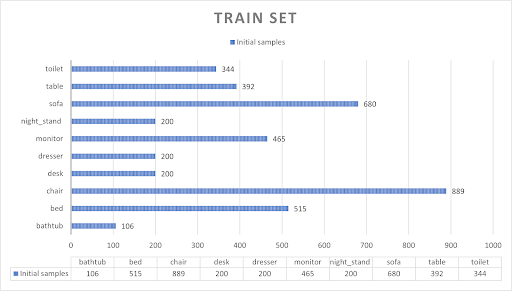
\includegraphics[scale = 0.45]{resources/distribution.png}
	\label{fig:initialTrainSetDistribution}
\end{figure}
In Figure \ref{fig:initialTrainSetDistribution} we can see the initial distribution of the training samples.
\   \\\\
\textbf{2) Pre-processing} 

The CAD models are in Object File Format (OFF), but our model, described in the session V. LEARNING FRAMEWORK, requires 3D boolean vectors with dimensions of \mbox{$32\times32\times32$}.

In order to get the required input format, we have done the following steps:
\begin{itemize}
	\item With the help of the Open3d Python library, we converted each model in the dataset to voxel grids, 2D list of filled positions. As mentioned before, this saves space and in our case, we went from 2.17 GB to 311 MB. [ code with parameters of sample rates…]
	\item Finally, we translated each voxel grid to the actual \mbox{$32\times32\times32$} boolean array. The code is available in our Git repository. [...with np and o3d]
\end{itemize}

As we can see from Figure \ref{fig:initialTrainSetDistribution}, the ModelNet10 is not an Independent and Identically Distributed (i.i.d.) dataset. The assumption of I.I.D is central to almost all machine learning algorithms, and we tried to make our data as much as i.i.d in the following way:
\begin{itemize}
	\item Firstly, we normalized the data, from the previous step, by subtracting the mean and dividing by the standard deviation;
	\item Then, we augmented all the voxel grids with new rotations [TODO: add how] to increase the samples in the dataset;
	\item Finally, we randomly picked ~1k samples per category.
\end{itemize}
Figure \ref{fig:finalTrainSetDistribution} shows the distribution we get after these steps.
\begin{figure}[]
	\centering
	\caption{Final Train Set Distribution [TODO correctone]}
	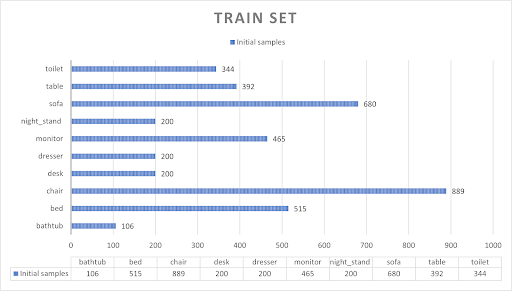
\includegraphics[scale = 0.45]{resources/distribution.png}
	\label{fig:finalTrainSetDistribution}
\end{figure}
\  \\\\
\textbf{3) Training Setup[RENAME]}

\MR{TODO: Last but not least, this section should also contain information on how you have split the dataset into training, validation and test sets. This will be briefly recalled within the ``Results'' section.}

\section{Learning Framework}
\label{sec:learning_framework}

Here you finally describe the learning strategy / algorithm that you conceived and used to solve the problem at stake. A good diagram to exemplify how learning is carried out is often very useful. In this section, you should describe the learning model, its parameters, any optimization over a given parameter set, etc. You can organize this section into \mbox{sub-sections}. You are free to choose the most appropriate structure.

\begin{remark}
Note that the diagram that you put here differs from that of Section~\ref{sec:processing_architecture} as here you show the details of how your learning framework, or the core of it, is built. In Section~\ref{sec:processing_architecture} you instead provide a high-level description of the involved processing blocks, i.e., you describe the {\it processing flow} and the rationale behind it.
\end{remark}

\noindent \textbf{On math typesetting:} there are many Latex tricks that you should use to produce a high quality technical essay. A few are listed below, in random order:
\begin{itemize}
\item \textbf{Vectors and matrices:} $x$ is a scalar, whereas $\bm{x}$ (in bold) is a vector, and $\bm{X}$ is a matrix with elements $\bm{X} = [x_{ij}]$. For bold symbols you may use the \texttt{\textbackslash bm} Latex command, e.g., \texttt{\textbackslash bm(x)}.
\item \textbf{Operators:} such as $\max$, $\min$, $\arg\!\max$, $\arg\!\min$ and special functions such as $\log(\cdot)$, $\exp(\cdot)$, $\sin(\cdot)$, $\cos(\cdot)$ are obtained through specific latex commands \texttt{\textbackslash min}, \texttt{\textbackslash max}, \texttt{\textbackslash arg\textbackslash!min}, \texttt{\textbackslash arg\textbackslash!max}, \texttt{\textbackslash log}, \texttt{\textbackslash exp}, \texttt{\textbackslash sin}, \texttt{\textbackslash cos}, etc. Use them! $log$, $exp$, $min$, $sin$, $cos$, etc., look ugly.
\item \textbf{Sets} can be represented through calligraphic fonts, e.g., $\mathcal{S}$, $\mathcal{F}$, $\mathcal{B}$, etc., obtained using the Latex command \texttt{\textbackslash mathcal{\{S\}}}, etc.
\item \textbf{Equations:} for a single equation use the \texttt{equation} Latex environment. Example: 
\begin{equation}
\label{eq:sigmoid}
\sigma(x) = \frac{1}{1+e^{-x}}.
\end{equation} 
Now, using round brackets $($ and $)$ we get
\begin{equation}
\label{eq:sigmoid_comma}
\sigma(x) = (\frac{1}{1+e^{-x}}),
\end{equation} 
but this looks ugly, you should use ``\texttt{\textbackslash left (}'' for ``$($'' and ``\texttt{\textbackslash right )}'' for ``$)$'', obtaining
\begin{equation}
\sigma(x) = \left ( \frac{1}{1+e^{-x}} \right ).
\end{equation} 
\item \textbf{Punctuation:} Displayed equations are usually considered to be part of the text and, in turn, they will get the very same punctuation as if they were inline with the text (and part of the sentence). If the sentence ends with a displayed equation, the equation gets a period ``.'' right after it, see Eq.~(\ref{eq:sigmoid}). iI the equation is instead part of a running sentence, which is continued after it, then the equation may be ended by a ``,'' as in Eq.~(\ref{eq:sigmoid_comma}). Use the standard grammar rules and your good sense of flow to assess how equations should be punctuated, I usually read through as if they were plain text.
\end{itemize} 



% !TEX root = template.tex

\section{Results}
\label{sec:results}

In this section, you should provide the numerical results. You are free to decide the structure of this section. As a general ``rule of thumb'', use plots to describe your results, showing, e.g., precision, recall and \mbox{F-measure} as a function of the system (learning) parameters. You can also show the precision matrix. 

\begin{remark}
Present the material in a progressive and logical manner, starting with simple things and adding details and explaining more complex findings as you go. Also, do not try to explain/show multiple concepts within the same sentence. Try to \textbf{address one concept at a time}, explain it properly, and only then move on to the next one.
\end{remark}

\begin{remark}
The best results are obtained by generating the graphs using a vector type file, commonly, either \texttt{encapsulated postscript (eps)} or \texttt{pdf} formats. To plot your figures, use the Latex \texttt{\textbackslash includegraphics} command. Lately, I tend to use pdf more.
\end{remark}

\begin{remark}
If your model has hyper-parameters, show selected results for several values of these. Usually, tables are a good approach to concisely visualize the performance as hyper-parameters change. It is also good to show the results for different flavors of the learning architecture, i.e., how architectural choices affect the overall performance. An example is the use of CNN only or CNN with adversarial training, or using residual layers for CNNs, dropout for better generalization or autoencoder models. So you may obtain different models that solve the same problem, e.g., CNN, CNN+residual layers, etc.
\end{remark}


% !TEX root = template.tex

\section{Concluding Remarks}
\label{sec:conclusions}
% What I would like to see here is:
% 1) a very short summary of what done,
% 2) some (possibly) intelligent observations on the relevance and applicability of your algorithms / findings,

The solution proposed in this paper provides a good accuracy, moreover we found  several advantages compared with a standard CNN model.

First, the memory requirements problem related to the Voxel grid is mitigated. 
%Since each weak model can be trained alone, we required to keep in memory only a portion of the dataset at a time. 
The solution implemented is very scalable, i.e. there are no specific constraints on the number of weak models, even if it's suggested to choose this number based on the availability of data. 

The execution of the whole system is also dynamic and can be adapted based on the potentiality of the computer in which it is executed. 
% 3) what is still missing, and can be added in the future to
% extend your work.
%In fact, since we use many small models that may run in parallel, the final prediction time may be lower than the amount of time required for the execution of a single bigger neural network. 
The model created can still be improved and enhanced using a larger number of models, and a larger dataset. 
Beyond enlarging the dataset and the number of models used for the final prediction for the Bagging, we can use another type of ensembling, i.e. Boosting. In our opinion, with Boosting we can further improve the results by paying more attention to wrongly classified classes like desk, dresser, night\_stand and table.
Furthermore, we would also like to explore the potential of sparse CNN \cite{graham2017submanifold} and transformers \cite{mao2021voxel} in classification task, to capture also long-range context information.\\
% 4 & 5 required by professor:
% Moreover: being a project report, I would also like to see
% a specific paragraph stating
% 4) what you have learned, and
% 5) any difficulties you may have encountered.
% This report showcases the work of the authors from the University of Padua on Project 3 (3D Objects Classification) of the Neural Network and Deep Learning Course.
% Our goal was to create a solution to classify Voxelized 3D objects, using Machine Learning techniques and ModelNet10 dataset as our reference.

During the development of this project we had possibility to develop the models on both, keras and pytorch, and we found that keras is much beginner-friendly than pytorch.
Another remark is that python libraries for 3D object manipulation are specialized for meshes and point clouds, but they don't provide full functionalities to work with voxel grid, we tested \textit{\href{http://www.open3d.org/}{open3d}} and  \textit{\href{https://trimsh.org/index.html}{trimesh}}, the popular ones. Even though Trimesh has more functions to work with voxels, the exportation of the voxel grids is not fully supported, so we used open3d for this project.
Finally, we trained our models on Colab and Kaggle, one of the free platforms that provide free GPU for the training, and we found that with colab is easier to connect with drive thus easier to comunicate between the notebook and drive itself for exchanging data. On the other hand, Kaggle provides different types of GPU and TPU. And for our bagging models, we trained the models in parallel, thus saving half of the training time.
% All the code is available in our Git repository at:  \mbox{\textit{\href{https://github.com/mrsingh-10/3d_classification}{https://github.com/mrsingh-10/3d\_classification}}}. \\

\section{Exam rules}

What you need to do to pass the exam:
\begin{itemize}
\item Optional: team up with another student. Max. group size is \textbf{three students} per group;
\item Identify a project to work on, devise your own neural network architecture and test it on the provided dataset;
\item \textbf{Prepare a written project report} including: i) diagrams, ii) configuration pars, iii) results, iv) your discussion;
\item \textbf{Prior to presenting your work}: upload i) your written report and ii) the code;
\item \textbf{Present your work} using slides (max. duration is 15 minutes): take turns in presenting your work, your individual contribution to the project should clearly emerge. 
\end{itemize}

Your final grade will be obtained taking into account the following criteria:
\begin{itemize} 
\item \textbf{Project} (50 points): originality (10 pt.) - data preprocessing techniques (10 pt.) - learning architectures (20 pt.) - comparison against other/existing approaches (10 pt.) 
\item \textbf{Written report} (25 points): clarity of exposition (8 pt.) - completeness (9 pt.) - analysis of results (number and type of metrics used) (8 pt.)
\item \textbf{Oral exposition} (25 points): duration (your talk must take max. 15 minutes, using slides) (15 pt.) - questions (10 pt.)
\end{itemize}

The final grade will be computed as
\begin{equation}
\textrm{grade} = \frac{\textrm{tot\_points} \times 30}{110}
\end{equation}

\bibliography{biblio}
\bibliographystyle{ieeetr}

\end{document}


